\section{Finite geometry and parameterization}\label{app:proofs}
These elementary arguments concern a common nonempty historical set $J$, an available rank $1\le j\le |J|$ and real arithmetic. Write $x=N_t$, $B=|x|$, $B_i=|N_i|$, and $d_{i,h}=N_{i+h}-N_i$, including $d_{i,0}=0$. The quantities $\ell_i=\min_h d_{i,h}$ and $u_i=\max_h d_{i,h}$ retain the notation of the main text.

\subsection{Common-set projection bounds}
Define $A_i=B+P_i-B_i$, $T_i=\max_h|x+d_{i,h}|$ and the floor projection $\Pi_B(v)=\max(B,v)$. Both $A_i$ and $T_i$ are at least $B$. A nondecreasing projection commutes with a finite order statistic, so $F_J=\Q(A)$, $S_J=\Q(T)$ and $K_J=\Q(\Pi_B(P))$. The projection is one-Lipschitz; therefore
\begin{equation}
|A_i-\Pi_B(P_i)|\le |B-B_i|,\qquad
|T_i-\Pi_B(P_i)|\le |x-N_i|.
\end{equation}
The second bound follows by applying the reverse triangle inequality to every path point, then taking the maximum and applying the floor projection. Order statistics are nonexpansive in the maximum paired-row difference: if $|a_i-b_i|\le R$ for each $i$, then $a_i\le b_i+R$ and conversely, which implies $|\Q(a)-\Q(b)|\le R$. Consequently,
\begin{equation}
|F_J-K_J|\le R_{\rm abs},\quad |S_J-K_J|\le R_{\rm signed},\quad
|F_J-S_J|\le R_{\rm abs}+R_{\rm signed},
\end{equation}
where $R_{\rm abs}=\max_{i\in J}|B-B_i|$ and $R_{\rm signed}=\max_{i\in J}|x-N_i|$. Among size-$m$ subsets, choosing the smallest signed distances minimizes their largest distance, since every other subset contains a distance at least as large as the $m$th ordered distance. This minimax statement concerns the signed radius. For any realized response, pinball loss is $\max(\tau,1-\tau)$-Lipschitz in its report, so the report bounds also bound absolute score differences. They supply no direction of score improvement and require common rows and rank.

\subsection{Envelope plateaus and signed anchors}
Put $v_i=-\ell_i\ge0$. The headroom of an increment envelope at anchor $z$ is
\begin{equation}
g_i(z)=\max(z+u_i,-z+v_i)-|z|
=\begin{cases}\max(u_i,v_i-2z),&z\ge0,\\\max(u_i+2z,v_i),&z\le0.\end{cases}
\end{equation}
The branches agree at zero. Thus $g_i$ is two-Lipschitz and lies between $\min(u_i,v_i)$ and $\max(u_i,v_i)$. Comparing $g_i(N_i)$ with $g_i(x)$ row by row and using order-statistic stability gives
\begin{equation}
|F_J-S_J|\le\max_{i\in J}\min\{2|x-N_i|,|u_i-v_i|\}.
\end{equation}
Symmetric envelopes, $u_i=v_i$, suffice for equality of $F_J$ and $S_J$. Nonnegative historical/query anchors and $u_i\ge v_i$ also suffice; the sign-reversed analogue interchanges the two envelope sides. These are sufficient conditions. The same range bound yields $F_J,S_J\le B+\Q\{\max(u_i,v_i)\}$. If every $B_i\le B$, then $F_J\ge K_J$; if every $B_i\ge B$, the order reverses. Both follow directly by comparing $A_i$ with $\Pi_B(P_i)$.

Equal absolute anchors can still leave a translated-path gap. Take $c>0$, $H=1$, $t=721$ and the history $N_s=(-1)^{s+1}c$. The completed pool $J=\{1,\ldots,720\}$ contains equal counts of both signs and the query is $c$. All native peaks are $c$ and all headrooms vanish. Raw translation gives half the peaks $c$ and half $3c$, so rank 685 yields $F=K=c$ and $S=3c$. Here $R_{\rm abs}=0$ and $R_{\rm signed}=2c$.

\subsection{Compatible futures with opposite score rankings}
Fix $d>0$ and an available corrected rank for a pool of size $n$. Set $t=H+n-1$, $N_s=d(t-s)$ through issue, and use origins $J=\{0,\ldots,n-1\}$. Every historical episode declines, giving $G_i=0$, while the current anchor is zero. Hence $F=0$ and $S=Hd$. A future staying at zero gives peak zero and strictly favors $F$; a continuation $N_{t+h}=-dh$ gives peak $Hd$ and strictly favors $S$. The identical observed history therefore permits either realized score ordering.

Report order can also differ across constructions. The artificial history $(0,-4,-1,2)$ with $H=1$ has completed origins $0,1,2$ and current anchor two. Their native peaks are $(4,4,2)$, headrooms $(4,0,1)$ and translated peaks $(2,5,5)$. At the available corrected rank three for $\tau=3/4$, this gives $F=6$, $S=5$ and $K=4$. This auxiliary quantile belongs only to the illustration.

\subsection{Fixed-coefficient residual replay}\label{app:replay}
Fix arbitrary $c,\phi$ and define residuals $\epsilon_s=N_{s+1}-c-\phi N_s$. Replaying a historical residual sequence from $x$ gives $M_{i,0}(x)=x$ and $M_{i,h+1}=c+\phi M_{i,h}+\epsilon_{i+h}$. Subtracting the observed recursion and using induction establishes
\begin{equation}
M_{i,h}(x)=N_{i+h}+\phi^h(x-N_i),\qquad
T^{\rm raw}_{i,h}(x)=N_{i+h}+(x-N_i).
\end{equation}
Taking absolute maxima and using the reverse triangle inequality gives
\begin{equation}
\left|\max_h|T^{\rm raw}_{i,h}(x)|-\max_h|M_{i,h}(x)|\right|
\le \max_{0\le h\le H}|1-\phi^h|\,|x-N_i|.
\end{equation}
For $0\le\phi\le1$, the coefficient is $1-\phi^H$; at $\phi=1$ the paths coincide. The identity is algebraic and needs no residual distribution. Treating historical blocks as representative future scenarios is an additional modeling premise. The replay's time order generally requires more information than the two raw increment extrema.

Horizon order alone leaves score effects unresolved. For example, $B=0$, both realized peaks equal one, the short report is ten, and the long report is one. Raising the long report to the short one changes its quantile loss from zero to $0.45$. This separates a known response floor from an ordering imposed between fitted reports.

\subsection{Peak parameterization of headroom regression}\label{app:ridge}
The current-magnitude predictor satisfies $B_i=\mu_{\kappa B}+\sigma_{\kappa B}z_{i,\kappa B}$ under the stated transform. Set
\begin{equation}
\alpha=\mu_{\kappa B}+s_\kappa\beta_0,\qquad
\theta=s_\kappa\beta+\sigma_{\kappa B}e_B.
\end{equation}
Positive homogeneity of pinball loss implies that multiplying the objective in \eqref{eq:qr} by $s_\kappa$ gives
\begin{equation}
\mathcal P_\lambda(\alpha,\theta)
=\frac1W\sum_{i\in\T}\rho_\tau(P_{i,H}-\alpha-z_{i,\kappa}^{\mathsf T}\theta)
+\frac{\lambda}{2s_\kappa}\|\theta-\sigma_{\kappa B}e_B\|_2^2.
\end{equation}
The issued report is $\max\{B_t,\alpha+z_{t,\kappa}^{\mathsf T}\theta\}$. The equivalent peak problem thus has a shifted slope penalty. For every response $P\ge B$, raising a report below $B$ to $B$ weakly reduces its realized pinball loss. Translation by a known $B$ also translates the corresponding conditional quantile. These finite relationships leave estimation and future calibration as separate questions.

\subsection{Elementary quantile scores}\label{app:murphy}
For a threshold $\eta$, the elementary score for forecast $c$ and outcome $p$ is
\begin{equation}
S_{\eta,\tau}(c,p)=\{\mathbf1(p<c)-\tau\}\{\mathbf1(\eta<c)-\mathbf1(\eta<p)\}.
\end{equation}
\citet{ehm2016} represents quantile-consistent scores as nonnegative mixtures of these elementary scores under the appropriate regularity conditions. The empirical difference is constant between forecast/outcome breakpoints, with equality conventions checked at the breakpoints. Both named primaries take positive and negative values over the full breakpoint set. Figure~\ref{fig:murphy} displays a reduced plotting grid; the sign audit uses all breakpoints. The crossing establishes absence of empirical uniform dominance over consistent scores; it supplies no population dominance test.

\begin{figure}[htbp]
\centering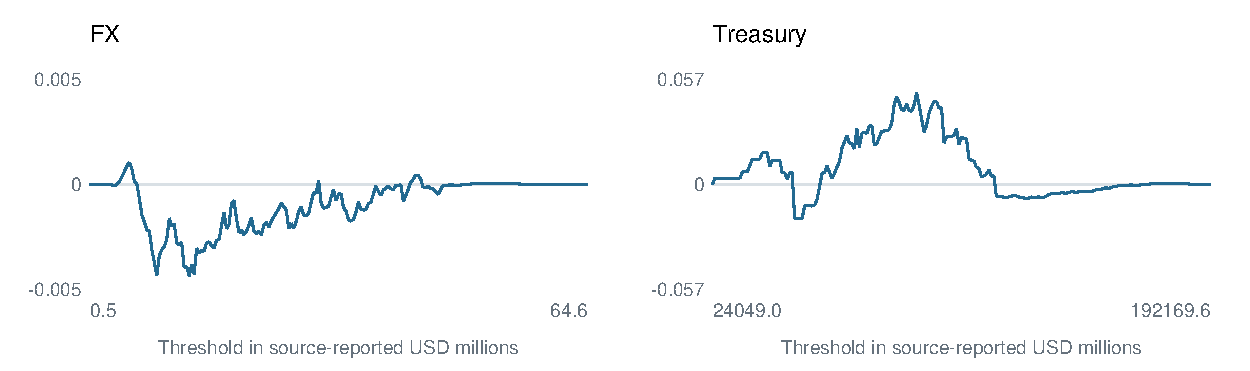
\includegraphics[width=\linewidth]{figures/murphy.pdf}
\caption{Elementary-score differences for the two original primaries, regression minus its declared reference. Positive and negative segments occur in each panel. Thresholds follow the respective source scales; the plotting subset preserves the audit's full-range sign conclusion.}\label{fig:murphy}
\end{figure}

\section{Earlier construction evidence}
Table~\ref{tab:old} retains the original historical-rule grid. $R$ is the symmetric-increment-envelope rule and $C^{\rm floor}=B$ is the issue-floor report. The earlier one-state retrieval study then compared recent and nearest signed-state pools. Its nearest native-peak improvement left the stronger original $F/S$ references ahead. The complete retrieval menu, monthly subdivisions and stationary-block sensitivities remain in the original result supplement; they are historical evidence from this same record.

\begin{table}[!htbp]
\centering\small
\caption{Original historical construction grid; mean FX losses in USD millions.}\label{tab:old}
\begin{tabular}{lrrrrrr}
\toprule
Setting & $F$ & $S$ & $R$ & $K$ & $C^{\rm floor}$ & $F-S$ \\
\midrule
main & 0.442 & 0.451 & 0.528 & 0.926 & 1.814 & -0.009 \\
h12 & 0.593 & 0.605 & 0.690 & 1.059 & 2.951 & -0.012 \\
h24 & 0.777 & 0.748 & 0.803 & 1.198 & 4.631 & +0.029 \\
n480 & 0.450 & 0.461 & 0.533 & 0.885 & 1.814 & -0.011 \\
n1440 & 0.444 & 0.448 & 0.527 & 0.932 & 1.814 & -0.004 \\
tau90 & 0.660 & 0.659 & 0.763 & 1.477 & 1.718 & +0.000 \\
tau99 & 0.155 & 0.159 & 0.175 & 0.289 & 1.890 & -0.004 \\
\bottomrule
\end{tabular}
\par\smallskip\begin{minipage}{\linewidth}\footnotesize Each sensitivity changes one factor from the original six-step setting. All rows retain the same evaluation issues; different score preferences are separate tasks. The displayed +0.000 in the tau90 row is positive before rounding.\end{minipage}
\end{table}


\FloatBarrier\clearpage
\section{Reproducibility and technical supplement}\label{app:repro}
The \href{https://github.com/ByronLi0207/financial-mathematics-paper-20261020}{repository} separates frozen original results, new exploratory results and document sources. The original working paper remains available beside this revision. The revision guide maps each current table and figure to its source file, records moved material, and provides the exact compilation command. Conventional bibliography entries replace reading-log annotations; the underlying source-evidence notes preserve consulted versions and ranges.

Exact recomputation requires the pinned source snapshots, model specification and code. The Treasury snapshot is archived with source attribution and terms. The FX acquisition route is documented separately; source redistribution rights remain unresolved. Public new outputs contain aggregates and numerical diagnostics, while per-origin financial arrays remain private. A later download of the same series can differ from the frozen version.

The original ridge optimizer uses two-block ADMM \citep{boyd2011}. Acceptance requires finite calculations, the declared primal/dual residual conditions and a feasible-dual objective-gap check. Its floating-point gap certificate bounds optimization error in the stated objective, rather than statistical adequacy or issued-report stability. An unpenalized intercept can have a flat minimizer interval: at real $\tau=19/20$, nineteen zeros and a single positive value $M$ admit every intercept in $[0,M]$. The implementation documentation retains the dual construction, iteration limits, tolerances and resource checks.

E1--E4 form a later exploratory supplement. The inference audit records the fixed Holm family, bandwidth sensitivity and coverage initialization correction. E3 records its pre-run menu and resource limits, original candidate eligibility, exact tie handling and all outcomes. The earlier four-predictor outputs were reused after reconciliation with their stored arrays and validation selections. These checks establish what was computed on the retained inputs; they add no independent financial sample.

The former long coverage-evidence table, full loss-weight frontiers, machine diagnostics and execution histories remain in their original repository paths. The \href{https://github.com/ByronLi0207/financial-mathematics-paper-20261020/tree/main/results}{result archive} retains adverse cells and original file identities. New coverage diagnostics supplement those records. The new manuscript is compiled directly from the delivered TeX using the bundled Tectonic engine, and the supplied PDF is that compiler's output.
